% \chapter*{\Huge Big Title Here}
% \addcontentsline{toc}{chapter}{Big Title Here}  % Add to TOC if needed

\chapter{Foundational structures: diagnosis and prognosis experts} % Main chapter title



%----------------------------------------------------------------------------------------
%	SECTION 
%----------------------------------------------------------------------------------------

\section{Introduction}
%-----------%-----------
%	SOUS-SECTION 
%-----------%-----------
\subsection{Elements of context}

\begin{itemize}
    \item Un premier modèle mécaniste avait été développer pour etudier la propagation et l'effet des lots sur le control des BRD. il suppose que l'infection est initié par un pathogène moyen donc les effets spécifiques des pathogènes sont moyennés. Ce modèle n'a jamais été fitté sur des observations réelles et donc on connaît pas s'il peut permettre d'expliquer des observations réels de vétérinaires. 
    \item Le protocol expérimental mis en place dans le cadre du projet SEPTIME (see originality of this thesis) a permis la collecte de données de format diverse à différente échelle de temps (fréquent vs ponctuel) et d'espace (individuel vs collectif). Il y a question sur quel proxy utilisé pour évaluer le deep et les modèles méca .
    % Comme première données, nous avons commencé par les vidéos d'échograhie pulmonaires. Parmis les sources de données collectées et vu qu'on parle maladie respiratoires, on a supposés que c'est un proxie direct pour informer de l'état des poumons.  
\end{itemize}


\subsection{Article originality}

%-----------
%	SOUS-SOUS-SECTION 
%------------
\subsubsection{Titre de la sous-sous-section}


\begin{itemize}
    \item Dans ce chapitre, nous nous sommes intérressés à la question  suivante: à partir d'une observation de capteur, peut-on automatiser le diagnostique avec un modèle deep learning et paramétrer indépendement un modèle mécaniste (pour le prognostique) de BRD sur des observations vétérinaire. (décrire la structure du deep et du modèle méca) et des objectifs spécifiques.
    \item Pour ces travaux nous avons choisir d'evaluer les performances de data-mining du deep sur des données d'échographie pulmonaires. Ce sont des données non-structurées, bruitées et on a supposés à priori que ce sont de bon proxies pour informer de l'état intérieur des poumons vu qu'on parle de maladie respiratoire.
    Les données ont étés prises sur t jours (rédecrire le protocol), il y'avait au total une trentaine de vidéos, annotée à partir de résultats d'examen clinique (animal cliniquement malade ou non).  (mettre une image). la quantité d'observations est limitée, prendre des échographies pulmonaires nécessite de déplacer les animaux et le vétérinaire et il faut raser l'endroit à scanner, parfois les animaux sont agités. En depis la quantité de données, nous avons voulu obtenir des méthodes qui fonctionnent.
\end{itemize}


%-----------%-----------
%	SOUS-SECTION 
%-----------%-----------
\subsection{Main contributions and perspectives}


\begin{itemize}
    \item nous avons entrainé un modèle de deep capable prédire l'état de santé clinique (symptomatique ou asymptomatique) à partir d'une vidéo d'echographie. Malgré une précision de 72\%, elle pourrait permettre d'automatiser le diagnostique et donner une approximation de la dynamique obsersée.
    \item nous avons paramétré un modèle epidémiologique de BRD sur les observations vétérinaires ce qui a permis de predire la dynamique à une grande echelle temporelle (prognostique) avec une RRMSE inférieur à 10\%. 
    \item nous avons généré un jeu réel de données vidéo d'échographie et annotations vétérinaire (symptomatique ou asymptomatique)
\end{itemize}

In the forecast of dynamics of BRD, with the limited amount of data, this work shows that deep learning could automate the diagnosis of particular data points in the time series. Independently, if using informative enough diagnosis, we can specify a mechanistic epidemiological model to fit particular data points and explicit the dynamics of BRD. In the next chapter, we answer the question of knowing how to choose the most likely mechanistic model amongst others based solely on observations of an outbreak in order to improve decision-making benefits.


\subsection{[In French] Résumé grand public}

%-----------------------------------
%	SECTION 
%-----------------------------------
\section{Proceedings published in Society for Veterinary Epidemiology and Preventive Medicine, 2024}

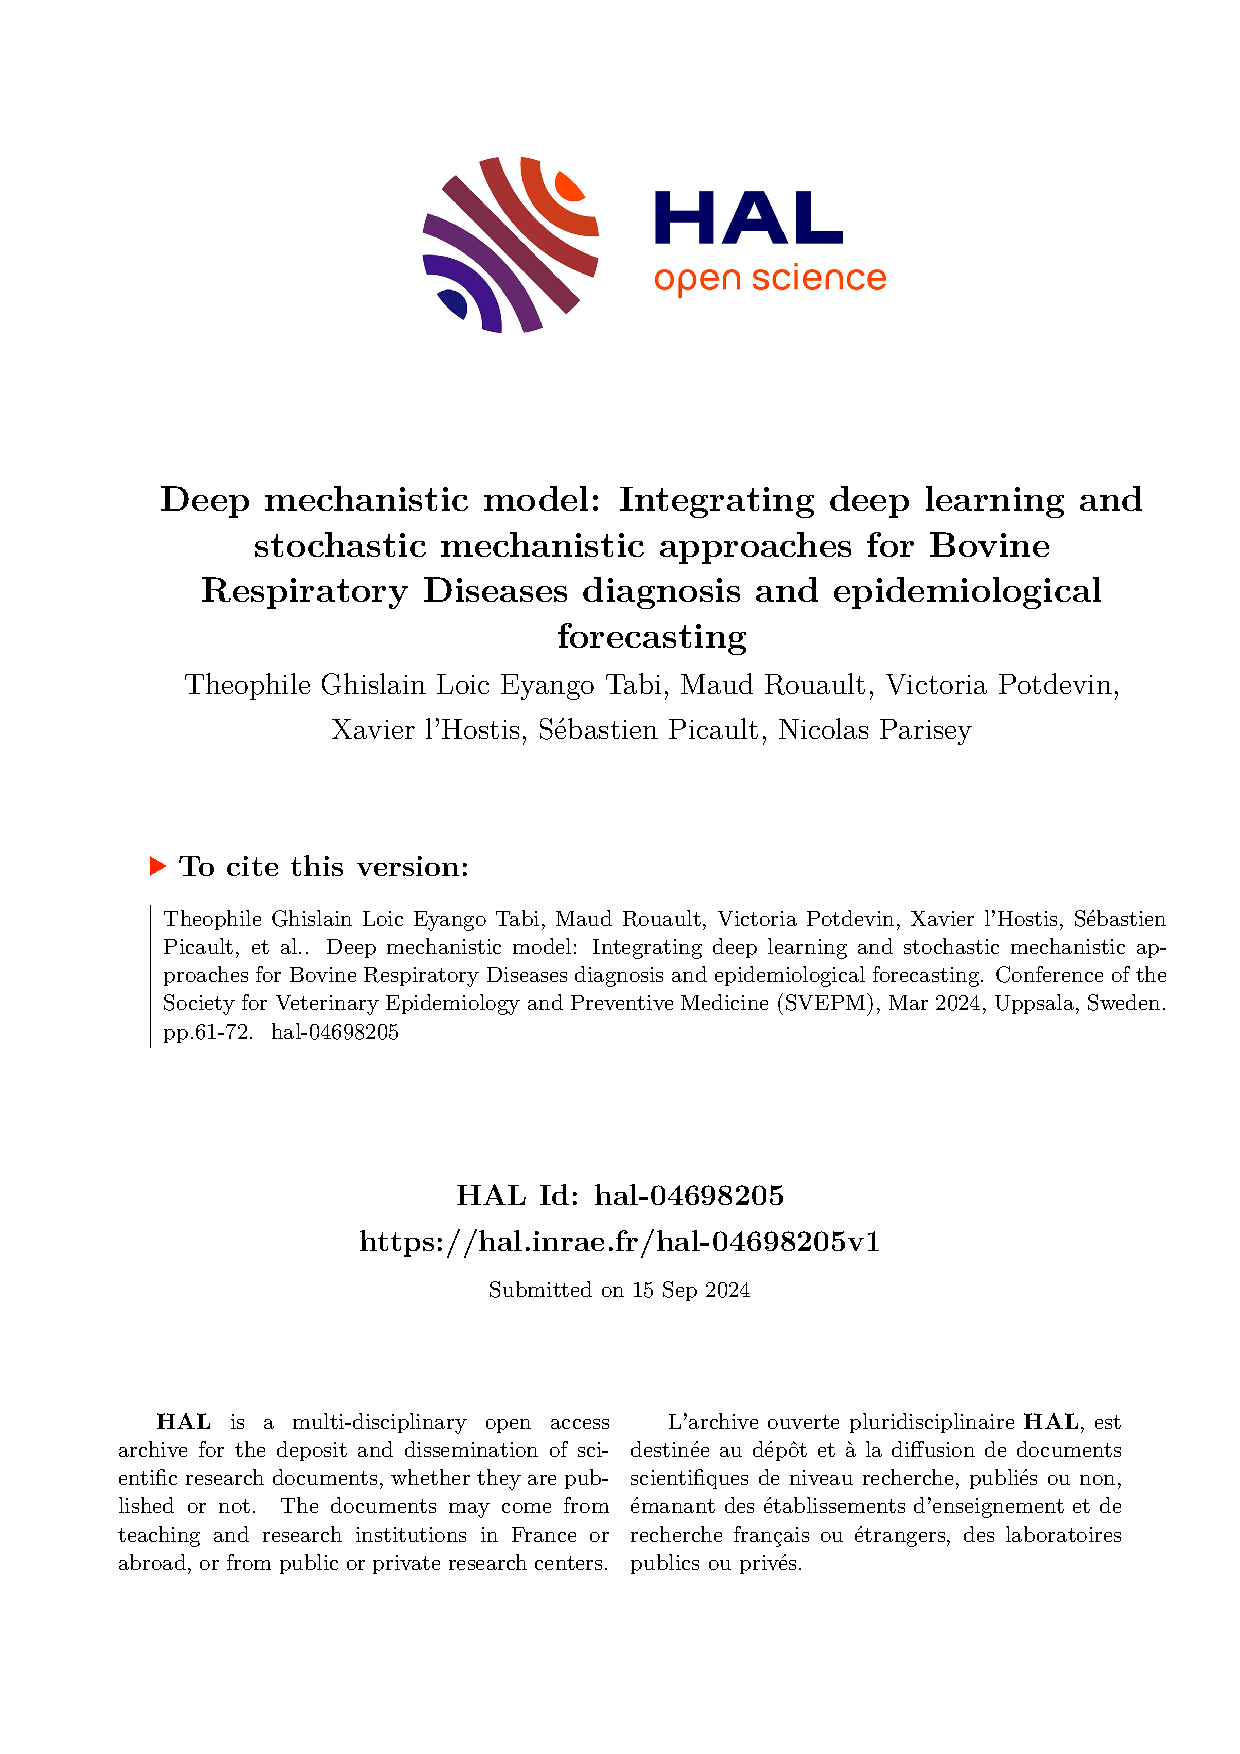
\includepdf[pages=-]{articles/SVEPM.pdf}  % Replace with your actual filename


